\chapter{Cadre général du stage}

\section*{Introduction}
\addcontentsline{toc}{section}{Introduction}


Dans ce chapitre, on va présenter le cadre général de notre project. on va d'abord présenter l'entreprise d'accueil, ensuite on va définir le cadre de ce projet de fin d'études à travers l'analyse de l'existant et la présentation de la problématique ainsi que la solution proposée, et enfin on va détailler la méthodologie de conception adoptée.
\section{Présentation de l'organisme d'accueil}
L'entreprise d'accueil est Billcom Consulting, une société de services et de conseil fondée en 2007, Billcom est spécialisée dans l'accompagnement des opérateurs de télécommunications par l'intégration des solutions BSS dont la gestion de la relation client et de la facturation, ainsi que la migration de données.
Basée en Tunisie, l'entreprise exerce ses activités auprès de clients situés à l'international, notamment en Afrique, au Moyen-Orient et en Europe.

\begin{figure}[H]
    \centering
    
\includegraphics[width=0.223\textwidth]{images/billcom-logo-2.png}
    \caption{Logo de la société d'accueil}
    \label{fig:billcom-logo}
\end{figure}

\begin{table}[H]
    \centering
    \renewcommand{\arraystretch}{1.3}
    \begin{tabular}{|>{\bfseries}l|l|}
        \hline
        Raison sociale & Billcom Consulting \\
        \hline
        Forme juridique & SARL \\
        \hline
        Adresse & Rue des Orangers Hammam Sousse \\
        \hline
        Téléphone & 58597507 \\
        \hline
        E-mail & contact@billcom-consulting.com \\
        \hline
        Secteur d'activité & Conseil et intégration de solutions télécoms \\
        \hline
    \end{tabular}
    \caption{Fiche d'identification de l'entreprise d'accueil}
    \label{tab:organisme_accueil}
\end{table}
\subsection{Services et domaine d'activité}

Afin de mieux présenter le domaine d'activité de Billcom Consulting, on va citer les services et les solutions offerts par cette société :

\begin{itemize}
    \item \textbf{Inégration des solutions de facturation et gestion client :}  déployer et maintenir des systèmes de gestion des abonnés (Customer Care) et des systèmes de facturation, incluant notamment les solutions technologiques de type BSS.

    \item \textbf{Business Consulting :} accompagner les clients dans l'analyse de leurs besoins, l'étude de leurs processus et le choix de solutions techniques et fonctionnelles cohérentes avec leurs objectifs.

    \item \textbf{Support technique :} assurer le support technique, la maintenance des solutions en place et l'assistance aux utilisateurs afin de garantir la continuité de service.

\end{itemize}
\subsection{Clients et collaborateurs}
Billcom Consulting s’est bien positionné sur le marché en fidélisant de nombreux clients. Parmi ceux-ci, on cite :
\begin{figure}[!htbp]
    \centering

\includegraphics[width=\textwidth]{images/clients.png}
\caption{Les clients de Billcom Consulting}
    \label{fig:Les clients de Billcom Consulting}
\end{figure}
\vspace{-0.5cm}
\section{Cadre du projet}
\subsection{Contexte global du projet}
Les opérateurs télécoms s'appuient sur des systèmes d'information complexes pour gérer l'ensemble du cycle de vie de leurs offres et services. Ces systèmes couvrent plusieurs processus métiers essentiels, notamment la gestion des clients, l'abonnement aux offres, le suivi de la consommation, la facturation et le recouvrement.
\newline
\newline
Avec l’évolution des besoins (nombre d’utilisateurs, diversité des offres, intégration avec d’autres systèmes), ces plateformes deviennent de plus en plus complexes à maintenir et à faire évoluer.


\subsection{Étude de l'existant}
Afin de justifier pleinement les choix architecturaux et technologiques opérés dans la création de notre application de gestion des services commercials, il est essentiel d'anlayser les systèmes actuellement utilisés chez les opérateurs télécoms.
\newline

Pour éviter de développer ces systèmes complexes en interne, la majorité des opérateurs se tourne vers des éditeurs logiciels spécialisés proposant des suites BSS prêtes à l'emploi. 
Dans cette approche, l'ensemble des modules décrits précédemment (CRM, Catalogue, Boutiques, Consommation, Facturation, Paiement) est compilé et regroupé au sein d'une seule et même application massive. 
\newline
On cite quelques solutions similaires:
\begin{itemize}
    \item[--] \textbf {Telkoware}
    \item[--] \textbf {Amdocs Kenan }
\end{itemize}
\begin{figure}[H]
    \centering
    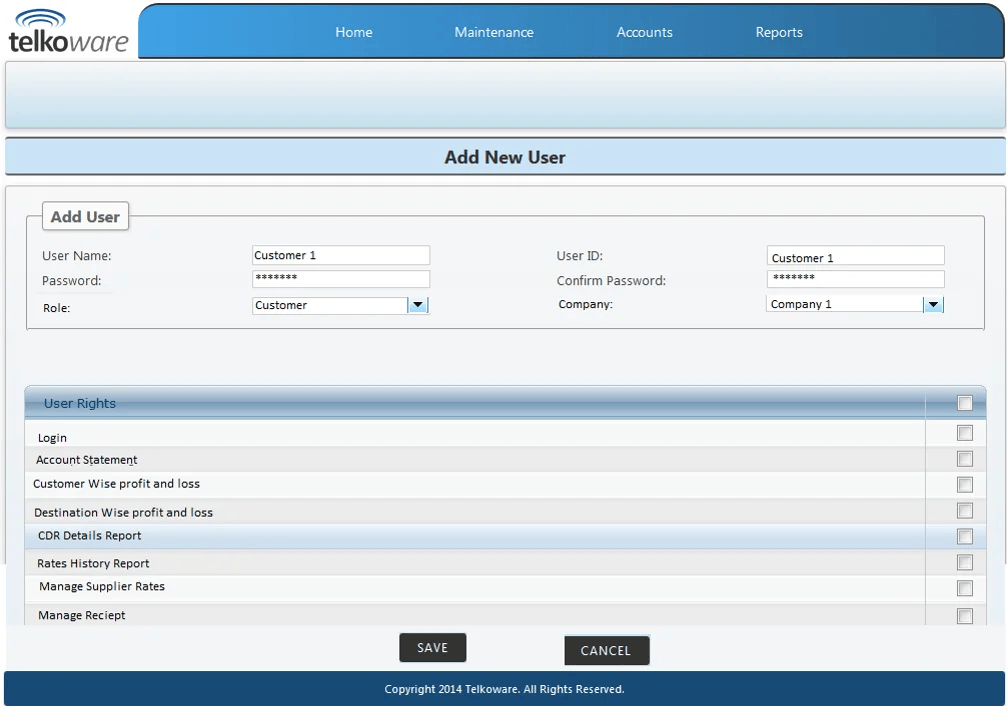
\includegraphics[width=0.9\textwidth]{images/BS-5.png.png}
    \caption{Interface de gestion client de la solution Telkoware}
    \label{fig:Telkoware}
\end{figure}

\subsection{Problématique}
Les équipes informatiques se retrouvent confrontées à plusieurs défis majeurs : la difficulté à livrer de nouvelles fonctionnalités rapidement sans perturber les opérations en cours et la difficulté de faire évoluer un composant du système de manière indépendante
\newline
Ces fonctionnalités sont souvent regroupées au sein de plateformes monolithiques centralisées.
Cette approche visait principalement à simplifier l'intégration initiale et à garantir la cohérence des données entre les différents modules métiers.

\subsection{Solution proposée}
Afin de répondre aux problématiques identifiées, une solution basée sur une architecture modulaire est proposée. Elle s’inspire des systèmes utilisés dans le domaine des télécommunications (BSS), tout en restant adaptée à un contexte de projet de fin d’études.
\newline 
La solution consiste à développer un système organisé en modules indépendants couvrant les principales fonctionnalités métier, notamment la gestion des clients, la gestion des services et des abonnements, la facturation, ainsi que le suivi via un tableau de bord.
Dans ce contexte, on a pensé à des interfaces simples et des actions faciles à utiliser en réduisant la navigation.
\newline
\vspace{-0.5cm}

 Les enjeux de ce projet sont l'automatisation, l'intégration du code ainsi que la livraison continue.
 L'objetif est de mettre en place un pipeline CI/CD, puis le déploiement de l'application dans un cluster Kubernetes, ainsi que l'implémentation d'une partie de surveillance(monitoring) de l'application en environnement de produciton.
 Ce projet s'inscrit dans une démarche DevOps, il constitue quatres phases principales: 
 \begin{itemize}
    \item[•] \textbf{Développment de l'application}
    \item[•] \textbf {Intégration continue / Livraison continue}
    \item[•] \textbf{Déploiement de l'application dans un cluster Kuberentes}
    \item[•] \textbf{Monitoring et alerting}
 \end{itemize}

\section{Langage de modélisation UML}
UML signifie "Unified Modeling Language" ou "Langage de Modélisation Unifié" en français. C'est un langage de modélisation graphique utilisé pour visualiser, spécifier, construire et documenter les systèmes logiciels. UML fournit un ensemble de notations et de diagrammes standardisés qui permettent de présenter le logiciel.
\newline
Il est composé de trois types de diagrammes (diagrammes statiques, diagrammes de comportement et diagrammes dynamiques), chacun ayant une fonction spécifique pour représenter différents aspects du système. Parmi les types de diagrammes les plus couramment utilisés, on trouve : \newline
Les diagrammes de classes, les diagrammes de cas d'utilisation, les diagrammes de séquence et les diagrammes d'activités.

\section{Méthodologie de travail}
Pour mener à bien le développement d'un projet informatique, il est très important de définir la méthode à suivre au cours du travail ainsi que les tâches à effectuer par la suite pour garantir un niveau de qualité acceptable et éviter les délais.

\subsection{Étude comparative des différentes méthodologies}
Le tableau suivant résume les différences entre l'approche classique et l'approche agile.

\begin{table}[H]
    \centering
    \renewcommand{\arraystretch}{1.3}
    \begin{tabular}{|>{\bfseries}p{3cm}|p{5.5cm}|p{5.5cm}|}
        \hline
        Thème & Approche classique & Approche agile \\
        \hline
        Cycle de vie & Séquentiel, en cascade. & Itératif et incrémental. \\
        \hline
        Planification & Définie dès le départ. & Adaptative et évolutive. \\
        \hline
        Documentation & Importante et détaillée. & Réduite au strict nécessaire. \\
        \hline
        Équipe & Rôles spécialisés, pilotage centralisé. & Équipe autonome et collaborative. \\
        \hline
        Changement & Résistance et gestion lourde. & Changement fréquent. \\
        \hline
        Validation & En fin de projet. & Continue, au fil des itérations. \\
        \hline
    \end{tabular}
    \caption{Tableau comparatif entre les méthodologies}
    \label{tab:comparaison_methodologies}
\end{table}
Après une étude comparative des méthodologies , présentées précédemment, nous
avons établi un tableau récapitulatif, illustré par le tableau 1.3 , qui contient les
avantages et les inconvénients de chaque méthode

\vspace{0.3cm}

\begin{table}[H]
    \centering
    \renewcommand{\arraystretch}{1.2}
    \begin{tabular}{|>{\bfseries}p{3.8cm}|p{5.5cm}|p{5.5cm}|}
        \hline
        Méthodologie & Avantages & Inconvénients \\
        \hline
        Classique & {\bfseries - Simple à mettre en oeuvre} \newline {\bfseries - Adaptée aux projets stables} & {\bfseries - Peu flexible} \newline {\bfseries - Spécifications figées dès le départ} \newline {\bfseries - Non adaptable à tout type de projet} \\
        \hline
        Agile & {\bfseries - Livraisons rapides} \newline {\bfseries - Meilleure adaptation aux besoins clients} \newline {\bfseries - Améliore la qualité d'exécution} & {\bfseries - Forte implication requise} \newline {\bfseries - Maîtrise de Scrum nécessaire} \newline {\bfseries - Non adaptable à tout type de projet} \\
        \hline
    \end{tabular}
    \caption{Avantages et inconvénients des méthodologies}
    \label{tab:avantages_inconvenients_methodologies}
\end{table}

\subsection{Choix de méthodologie - Scrum}
La méthode Scrum est une approche agile qu'on a adopté afin de garantir la flexibilité, l'efficacité et l'adaptabilité. Contrairement aux méthodes tradionnelles comme la méthodologie en V ou le modèle en cascade, l'agilité repose sur des cycles courts et itératifs, mieux adaptés aux projets évolutifs.
Elle suppose que le développement d'un logiciel n'est pas prévisibile et ne peut donc pas suivre de processus défini. Ainsi, le résultat du projet n'est pas déterminé au départ, il dépend des retours du client permettant de s'adapter aux imprévus et de maintenir une communication constante avec les parties prenantes.
\newline

La figure suivante présente le schéma décrivant les principes de la méthodologie Scrum. Le principe de base de Scrum est de diviser le projet sur un ensemble d'itérations à réaliser, appelées Sprints. Chaque Sprint possède des buts à atteindre, à partir desquels sont définies les fonctionnalités à implémenter.
Ces fonctionnalités sont définies dans un backlog de produit sous forme de User Stories, qui sont des descriptions courtes et simples d'une fonctionnalité du point de vue de l'utilisateur final.
Un sprint aboutit toujours à la livraison d'une version améliorée et partiellement fonctionnelle du produit appelée MVP.
\begin{figure}[H]
    \centering
    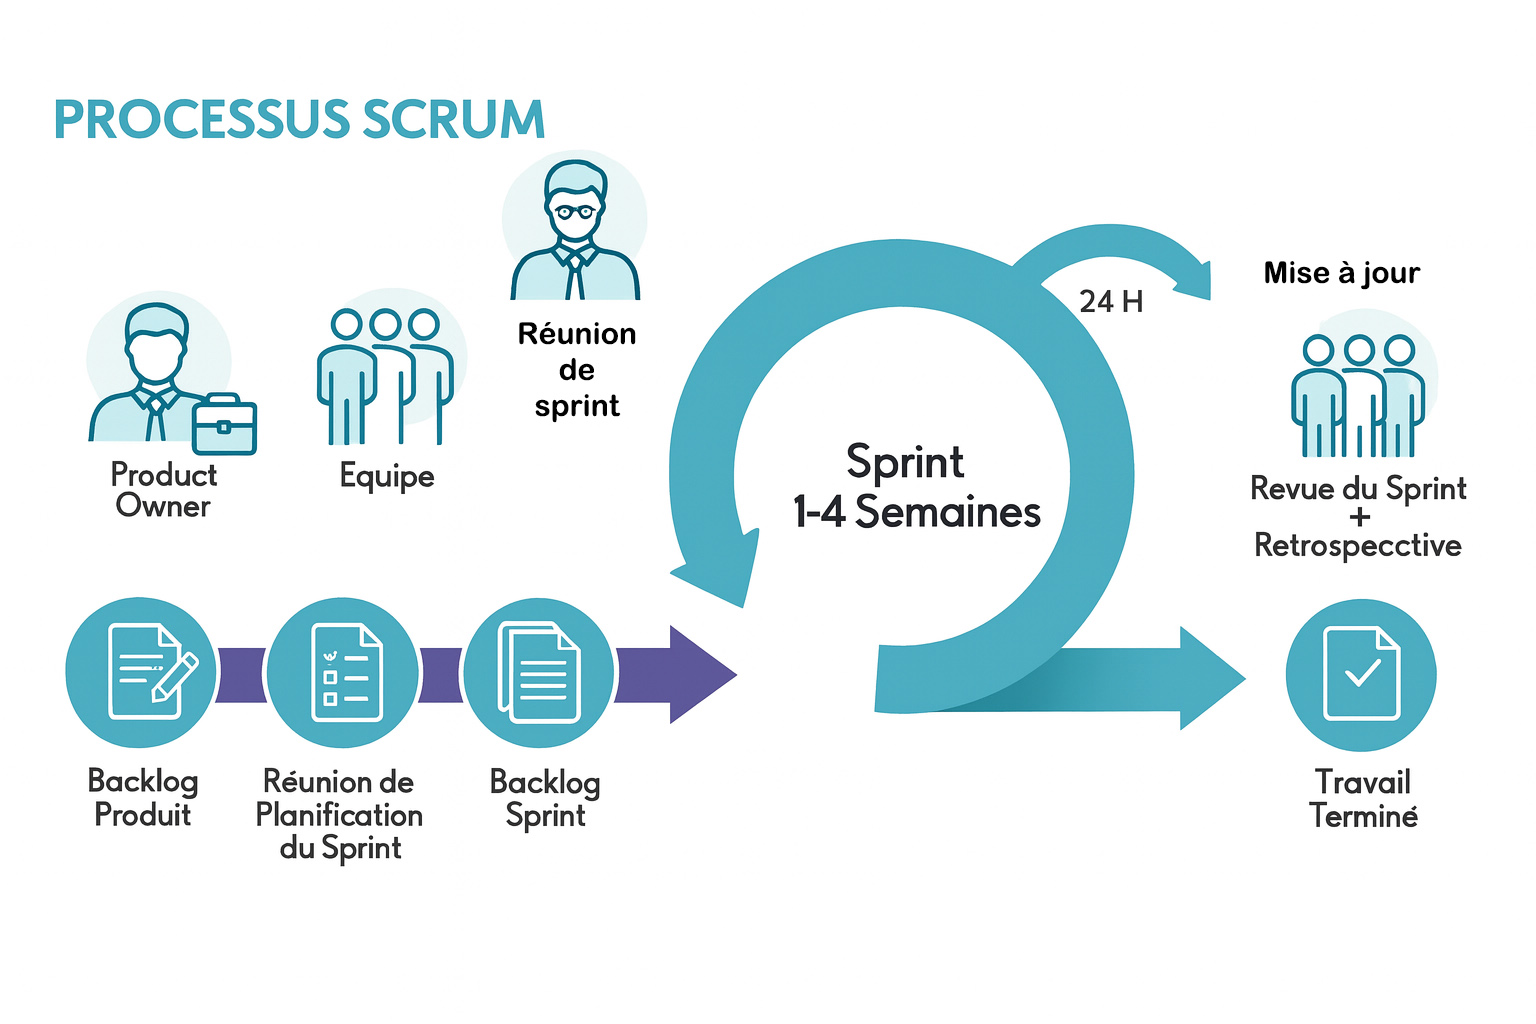
\includegraphics[width=0.8\textwidth]{images/processus-scrum.jpg}
    \caption{La méthodologie Scrum}
    \label{fig:Scrum}
\end{figure}
\subsubsection {Les rôles et les artefacts dans Scrum}
Les trois rôles principaux dans Scrum sont:
 \begin{itemize}
\item[•] \textbf{Product Owner :} il représente le client et les parties prenantes. Il est responsable de maximiser la valeur du produit  il en porte la vision métier. Il définit la feuille de route et gère le \textit{Product Backlog} : contenu, disponibilité et ordre de priorité des éléments.
\vspace{0.16cm}
\newline
\item[•]\textbf{Scrum Master :} il veille au respect du cadre Scrum et facilite son application au quotidien. Son rôle est d'accompagner le Product Owner et l'équipe de développement, de lever les obstacles et de favoriser l'amélioration continue. Ce n'est pas un chef de projet, même si les deux rôles peuvent parfois être cumulés selon le contexte.
\vspace{0.16cm}
\item[•]\textbf{Équipe de développement :} réalise un incrément livrable du produit à chaque Sprint selon les priorités définies. Elle est pluridisciplinaire et peut regrouper différents profils techniques, comme des développeurs, des architectes et des administrateurs de bases de données.
 \end{itemize}
 Les artefacts principaux de Scrum sont:
  \begin{itemize}
\item[•] \textbf{Product Backlog:} Une liste structurée de tous les requis, besoins du client et spécifications du produit. C'est le Product Owner qui est chargé de sa mise à jour tout au long du projet.
\item[•] \textbf{Sprint Backlog:} Un schéma précis des actions à réaliser au cours du Sprint.Il est conçu en début de chaque Sprint à partir du product backlog. Cela permet à l'équipe de surveiller l'avancement et de répondre aux objectifs établis par le Product Owner.
 \end{itemize}
%Maybe include a subsection about the ceremonies
\subsubsection{Justification du choix}
Le choix de la méthodologie Scrum fournit des avantages pour les clients, Scrum permet au client de tester et de valider les fonctionalités au fur et à mesure de leur développement ce qui permet d'obtenir un retour d'information rapide et de s'assurer que le produit final correspond aux attentes du client permettant de minimiser les problèmes de compréhension de la conception. En plus, le client peut ajouter ou modifier les fonctionalités pendant le sprint planning ou le sprint review. Ainsi, Scrum assure la qualité du produit livré.

\section*{Conclusion}
Dans ce chapitre, on a présenté l'entreprise d'accueil, le cadre général de notre projet. Par la suite on a proposé la solution adoptée suite à l'étude de l'existant. Enfin, on a détaillé la méthodologie de travail à suivre pour mener à bien le projet. 

\newpage
